%!TEX program = xelatex
\documentclass[cn,pad,11pt,geye]{elegantnote}

\title{\ttfamily《模拟电子技术基础笔记》}

\author{\href{https://github.com/sikouhjw}{死抠}}
%\institute{\href{https://elegantlatex.org/}{Elegant\LaTeX{} Program}}
\version{2.10}
\date{\today}
\hypersetup{
	bookmarks=true,
	bookmarksopen=true
}

\begin{document}
\maketitle
% logo
\centerline{
\includegraphics[width=0.25\textwidth]{logo}}

\setlist[itemize]{label=$\circ$}
\section{常用半导体器件}
\subsection{基本概念}
\begin{definition}[本征半导体]
	纯净的具有晶体结构的半导体称为本征半导体。
\end{definition}
\begin{note}
	本征半导体具有掺杂、热激活特性,即人为地掺入特定的杂质元素或在光照的条件下,其导电性会有明显的变化。
\end{note}
\begin{definition}[载流子]
	运载电荷的粒子称为载流子。
\end{definition}
\begin{note}
	本征半导体的载流子为自由电子和空穴,半导体在热激发下产生自由电子和空穴称为本征激发,逆过程称为复合。由于本征激发与复合是互逆过程,因此一定温度下的载流子浓度是一定的,并且载流子浓度与热力学温度近似成指数关系。多数载流子简称多子,少数载流子简称少子。
\end{note}
\begin{definition}[N(P)型半导体]
	在纯净的硅晶体中掺入五(三)价元素(如磷(硼)),使之取代晶格中硅原子的位置,就形成了N(P)型半导体。
\end{definition}
\begin{note}
	由于磷(硼)在掺入硅晶体后会产生自由电子(空穴),因此称其原子为施主(受主)原子。\\
	N:自由电子数(多子)=正离子数(掺杂)+空穴数(热激发)。\\
	P:空穴数(多子)=负离子数(掺杂)+自由电子数(热激发)。
\end{note}
\begin{definition}[扩散运动,偏移运动]
	由于浓度差而产生的运动称为扩散运动。在电场力作用下,载流子的运动称为漂移运动。
\end{definition}
\begin{note}
	多子的扩散运动会使空间电荷区\footnote{见定义\ref{kongjian}}变厚,少子的漂移运动会使空间电荷区变薄。
\end{note}
\begin{figure}[h]
	\centering
	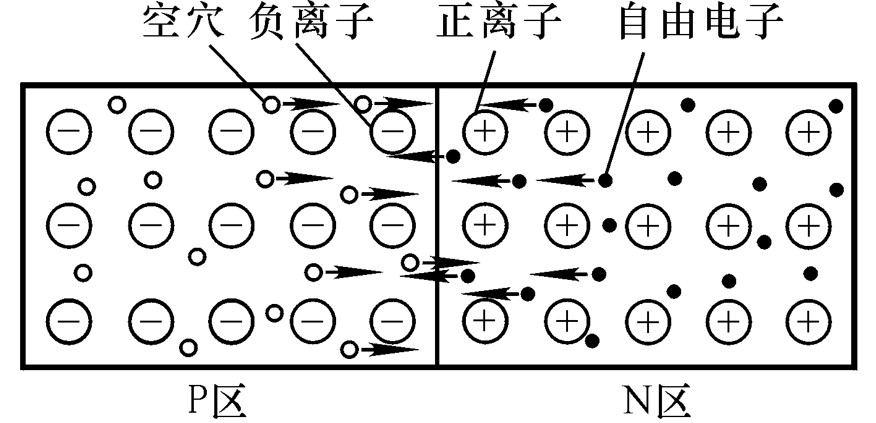
\includegraphics[width=0.6\textwidth]{PNjie1.jpg}
	\caption{扩散示意图}
\end{figure}

\begin{definition}[PN结]
	将P型半导体与N型半导体制作在同一块硅片上,其交界处会形成PN结。\label{kongjian}
\end{definition}
\begin{note}
	由于多子的扩散运动,硅片的交界处会有大量的载流子复合,交界处的载流子浓度下降,称此区域为空间电荷区(也称为耗尽区)。其电场性质主要受施主、受主原子影响,因此会产生内电场(由$N\to P$),阻碍多子的扩散运动(P区的空穴$\to N$,N区的自由电子$\to P$),促进少子的漂移运动(N区的空穴$\to P$,P区的自由电子$\to N$),从而最终达到稳态,形成PN结。
\end{note}
\begin{figure}[h]
	\centering
	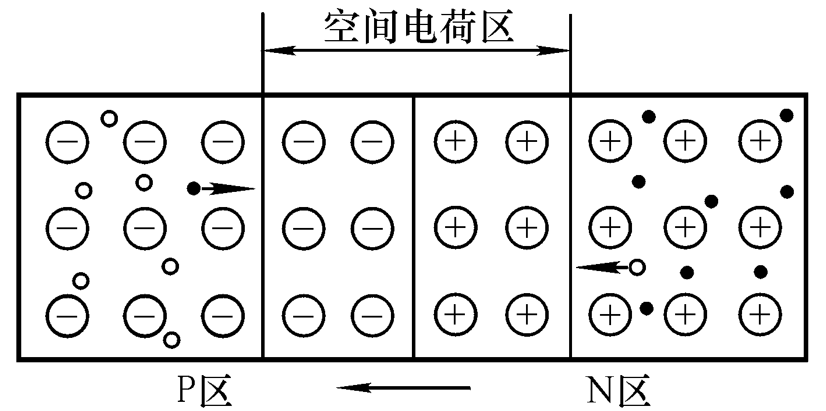
\includegraphics[width=0.6\textwidth]{PNjie2.png}
	\caption{PN~结示意图}
\end{figure}
\begin{definition}[PN结的正反接]
	将电源的正极接到PN结的P端,负极接到N端,则称此为正向接法(正向偏置)。反向接法则与之相反。
\end{definition}
\begin{proposition}[PN结的单向导电性]
	下面讨论在没有击穿\footnote{见性质\ref{jichuan}}的情况下正反接的情况
	\begin{itemize}
		\item 在正向接法中,由于空间电荷区等效的电源与外加电源方向相反
		\begin{itemize}
			\item 若外加电压大于内部电压,将会使空间电荷区消失,即PN结导通。
			\item 若外加电压小于内部电压,空间电荷区会变薄,仍不导电(近似)。
		\end{itemize}
		\begin{figure}[h]
			\centering
			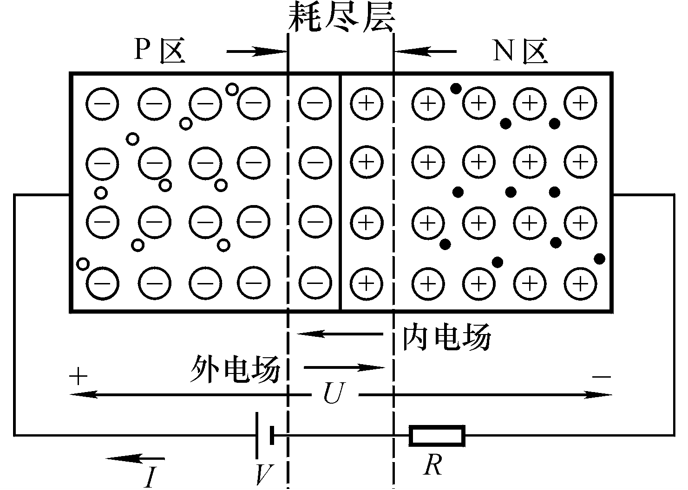
\includegraphics[width=0.4\textwidth]{PNjie3.png}
			\caption{正接示意图}
			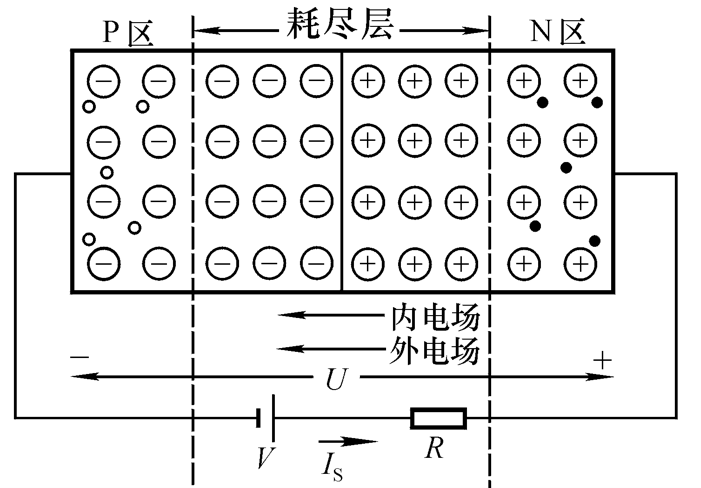
\includegraphics[width=0.4\textwidth]{PNjie4.png}
			\caption{反接示意图}
		\end{figure}
		\item 在反向接法中,由于空间电荷区等效的电源与外加电源方向同向,使空间电荷区变厚,内电场增强,形成漂移电流\footnote{少子的偏移运动产生的电流}。由于少子的数量极少,因此认为PN结反接时为截止状态且反向电流饱和。
		
	\end{itemize}
\end{proposition}
\begin{theorem}[PN结的电流方程]
	由理论分析可知,PN结所加端电压$u$与流过它的电流$i$的关系为$$i=I_{S}\left(\mathrm{e}^{\frac{qu}{kT}}-1\right)$$
	式中$I_S$为反向饱和电流,$q$为电子的电量,$k$为玻尔兹曼常量,$T$为热力学温度。作换元$U_{\mathrm{T}}=\frac{kT}{q}$得
	$$i=I_{S}\left(\mathrm{e}^{\frac{u}{U_{\mathrm{T}}}}-1\right)$$
	常温下(T=300K),$U_{\mathrm{T}}\approx26\mathrm{mV}$
\end{theorem}
\begin{proposition}[击穿电压]\label{jichuan}
	当外加电压过大时,PN结会被击穿,其中击穿又分可逆击穿与不可逆击穿。
	\begin{itemize}
		\item 可逆击穿(电流加以限制的情况下),称产生可逆击穿时的电压为击穿电压$U_{\textrm{BR}}$
		\begin{itemize}
			\item 齐纳击穿\footnote{在高掺杂的情况下,因耗尽层宽度很窄,不大的反向电压就可在耗尽层形成很强的电场,而直接破坏共价键,使价电子脱离共价键束缚,产生电子-空穴对,致使电流急剧增大。}
			\item 雪崩击穿\footnote{在掺杂浓度较低,耗尽层宽度较宽的情况下,当反向电压增加到较大数值时,耗尽层的电场使少子加快漂移速度,从而与共价键中的价电子相碰撞,把价电子撞出共价键,产生电子-空穴对。新产生的电子与空穴被电场加速后又撞出其它价电子,载流子雪崩式地倍增,致使电流急剧增加。}
		\end{itemize}
		\item 不可逆击穿——热击穿:不论是正接还是反接,当PN结消耗功率(UI)过大时,会产生大量的热量,致使元件烧坏。
	\end{itemize}
\end{proposition}
\begin{definition}[PN结等效的电容]\label{dianrong}
	具体内容跳转到\hyperref[disizhang]{第四章}
\end{definition}
\begin{definition}[半导体二极管]
	将PN结用外壳封装起来,并加上电极引线就构成了半导体二极管,简称二极管。
\end{definition}
\begin{case}
	二极管几种常见的结构
	\begin{itemize}
		\item 点接触型二极管(图(a)),适用于高频电路和小功率整流。
		\item 面接触型二极管(图(b)),适用于工频\footnote{工频就是一般的市电(工业用电)频率,在我们国家是50赫兹。工频是很低的频率。我国通常叫的工频,就是指50HZ的交流电。}大电流整流电路。
		\item 平面型二极管(图(c)),结面积较大的可用于大功率整流,结面积小的可作为脉冲数字电路中的开关管。
	\end{itemize}
\end{case}
\begin{figure}[h]
	\centering
	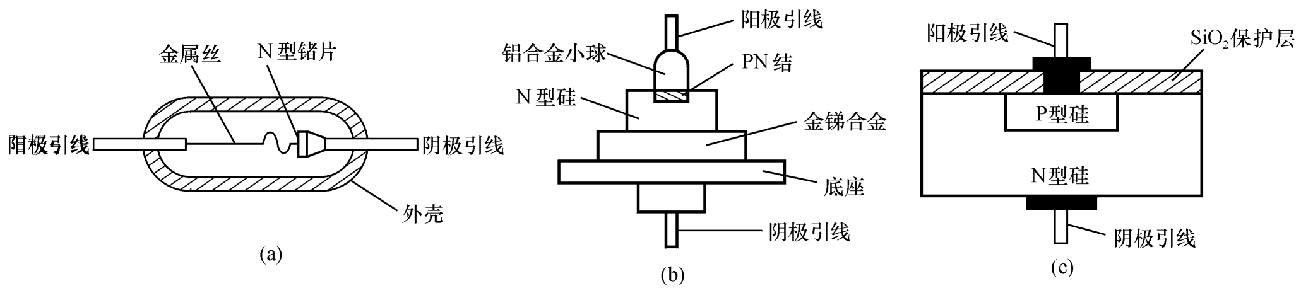
\includegraphics[width=1\textwidth]{erjiguan1.png}
	\caption{二极管常见类型}
\end{figure}
\begin{proposition}[二极管的伏安特性]下面给出二极管的几个性质
	\begin{itemize}
		\item 二极管与PN结伏安特性的异同
		\begin{itemize}
			\item 异
			\begin{itemize}
				\item 二极管导通后认为$U$近似不变(恒压)
				\item 二极管具有导通压降\footnote{即达到该电压后二极管彻底导通,电压不再变化}(通常硅管取0.7V,锗管取0.2V)
			\end{itemize}
			\item 同:都具有死区电压\footnote{死区电压,指的是即使加正向电压,也必须达到一定大小才开始导通,这个阈值叫死区电压}(通常硅管取0.5V,锗管取0.1V)
		\end{itemize}
		\item 二极管的伏安特性曲线如下,其中$U_{\mathrm{(BR)}}$是击穿电压,$I_{\mathrm{S}}$是反向饱和电流,$U_{\mathrm{on}}$是死区电压
		\begin{figure}[h]
			\centering
			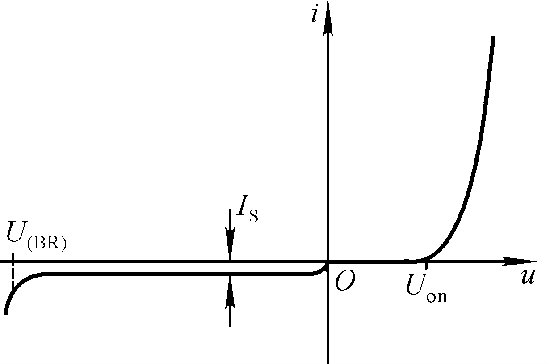
\includegraphics[width=0.4\textwidth]{erjiguan2.png}
			\caption{二极管伏安特性曲线}
		\end{figure}
		\item 温度对二极管伏安特性的影响:当温度升高时,二极管的正向特性曲线向左移(更容易导通),反向特性曲线向下移(少子增多,反向饱和电流变大)\label{wendu}
		\item 二极管的主要参数
		\begin{itemize}
			\item 最大整流电流$I_{\mathrm{F}}$:$I_{\mathrm{F}}$是二极管长期运行时所允许的最大正向平均电流,若超过$I_{\mathrm{F}}$二极管可能被热击穿。
			\item 最大反向工作电压$U_{\mathrm{R}}$:$U_{\mathrm{R}}$是二极管工作时所允许外加的最大反向电压,若超过$U_{\mathrm{R}}$二极管可能因反向击穿而损坏。$U_{\mathrm{R}}$通常取击穿电压$U_{\mathrm{(BR)}}$的一半。
			\item 反向电流$I_{\mathrm{R}}$:$I_{\mathrm{R}}$是二极管未击穿时的反向电流。$I_{\mathrm{R}}$越小说明二极管的单向导电性越好。$I_{\mathrm{R}}$对\hyperref[wendu]{温度}非常敏感。
			\item 最大工作频率$f_{\mathrm{M}}$:当电流频率超过$f_{\mathrm{M}}$,二极管将不能很好的体现单向导电性\footnote{见定义\ref{dianrong}}。
		\end{itemize}
	\end{itemize}
\end{proposition}
\begin{corollary}[二极管的等效电路]
	二极管的等效电路可以概括为三直一交
	\begin{itemize}
		\item 理想模型:导通时正向压降为0,截止时反向电流为0。
		\item 恒压降模型:只是将理想模型的导通点向右移了一个$U_{\mathrm{on}}$。(最常用)
		\item 折线模型:在恒压降模型的基础上增加了一个$r_0$直流电阻。(科研论文)
		\item 交流等效模型:在静态工作点附近加一微变量,其变化量用静态工作点的导数近似估计。
	\end{itemize}
\end{corollary}


\section{基本放大电路}
\section{集成运算放大电路}
\section{放大电路的频率响应}
\label{disizhang}

\begin{theorem}
	定理theorem
\end{theorem}
\begin{lemma}
	引理lemma
\end{lemma}
\begin{proposition}
	性质proposition
\end{proposition}
\begin{corollary}
	推论corollary
\end{corollary}
\begin{definition}
	定义definition
\end{definition}
\begin{conjecture}
	猜想conjecture
\end{conjecture}
\begin{example}
	例example
\end{example}
\begin{remark}
	评论remark
\end{remark}
\begin{note}
	注note
\end{note}
\begin{case}
	案例case
\end{case}

\section{放大电路中的反馈}
\subsection{反馈}
\begin{definition}
	反馈:将输出量的一部分作用到输入回路,用来影响输入量。
\end{definition}
\begin{note}
	反馈又有正负反馈、直交流反馈和本级级间反馈之分,这是显然的。
\end{note}
\begin{figure}[h]
	\centering
	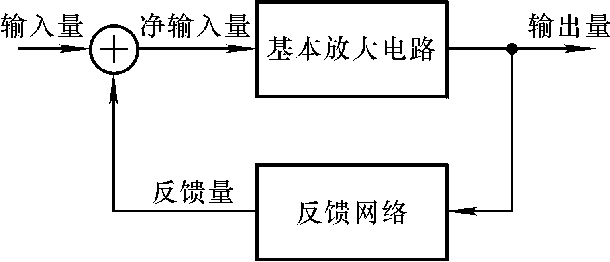
\includegraphics[width=0.5\textwidth]{fankui1.png}
	\caption{反馈电路示意图}
\end{figure}
\begin{note}
	判断反馈类型的经验方法:\\
	在输出端采样,一般为电压采样,在输出端上下方采样,一般为电流采样。\\
	反馈点与输入端不同端为串联反馈,同端为并联反馈。\\
	$\oplus-\oplus$\footnote{这里的$\oplus,\circleddash$应理解为前者是输入量,后者是反馈量,$\oplus$是正的,$\circleddash$是负的}常为串联,$\oplus+\circleddash$常为并联\\
	这是容易记忆的,只需判断是什么采样,是串联\footnote{以电压方式相叠加,反之亦然}或者并联反馈,再判断是正负反馈和交直流反馈,就可以组成名词:直流电压并联负反馈。
\end{note}
\begin{proposition}[关于负反馈]
	关于负反馈,它会使输出电阻产生变化,进而达到更好的产品要求。
	\begin{itemize}
		\item 电压负反馈:减小输出电阻 $\to$ 增强带负载能力。
		\item 电流负反馈:增强输出电阻 $\to$ 减小带负载能力。
	\end{itemize}
\end{proposition}
\subsection{方块图}
下面我们来分析一下负反馈电路的一般情况,即方块图。
\begin{figure}[h]
	\centering
	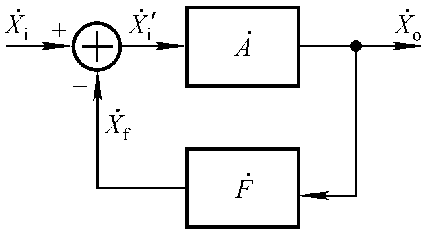
\includegraphics[width=0.5\textwidth]{fankui2.png}
	\caption{方块图示例}
\end{figure}

通过电路知识,我们容易得到以下几个等式
\begin{equation*}
	\dot X_\mathrm{i}'=\dot X_\mathrm{i}-\dot X_\mathrm{f}
\end{equation*}
\begin{definition}[基本放大电路的放大倍数]
	\begin{equation}
		\dot{A}=\frac{\dot{X}_{\mathrm{o}}}{\dot{X}_{\mathrm{i}}'}\label{eq:1}
	\end{equation}
\end{definition}

\begin{definition}[反馈系数]
	\begin{equation}
		\dot{F}=\frac{\dot{X}_{\rm{f}}}{\dot{X}_{\rm{o}}}\label{eq:2}
	\end{equation}
\end{definition}

\begin{definition}[负反馈放大电路的放大倍数(闭环放大倍数)]
	\begin{equation}
		\dot{A}_{\rm{f}}=\frac{\dot{X}_{\rm{o}}}{\dot{X}_{\rm{i}}}\label{eq:3}
	\end{equation}
\end{definition}

\begin{definition}[电路的环路放大倍数]
	\begin{equation}
		\dot{A}\dot{F}=\frac{\dot{X}_{\rm{f}}}{\dot{X}_{\rm{i}}'}\label{eq:4}
	\end{equation}
\end{definition}
根据公式~(\ref{eq:1})、(\ref{eq:2})、(\ref{eq:3})、(\ref{eq:4})可得
\begin{equation}
	\dot{A}_{\rm{f}}=\frac{\dot{A}}{1+\dot{A}\dot{F}}\label{eq:5}
\end{equation}
在中频带,公式~(\ref{eq:1})、(\ref{eq:2})、(\ref{eq:3})、(\ref{eq:4})、(\ref{eq:5})均为实数
分析~(\ref{eq:5})可得
\begin{table}[ht]
	\centering
	\begin{tabular}{cl}
		$AF>0$ & 负反馈\\
		$AF<0,AF\ne-1$ & 正反馈\\
		$AF=-1$ & 自激振荡\\
		$A+F\gg1$ & 深度负反馈
	\end{tabular}
\end{table}
\subsection{深度负反馈}
根据深度负反馈定义,我们可以得出这几个结论:
\begin{enumerate}
	\item 深度负反馈在分析中忽略净输入量,即$\dot{X}_{\rm{i}}=\dot{X}_{\rm{f}}\label{eq:6}$。当为串联负反馈时,忽略$\dot{U}_{\rm{i}}'$,即$\dot{U}_{\rm{i}}=\dot{U}_{\rm{f}}$。当为并联负反馈时,忽略$\dot{I}_{\rm{i}}'$,即$\dot{I}_{\rm{i}}=\dot{I}_{\rm{f}}$。
	\item 下面分析四种负反馈的反馈系数
	\begin{enumerate}
		\item 电压串联负反馈电路见图~\ref{tu:1},容易得到
		\begin{figure}[ht]
			\centering
			\subcaptionbox{电压串联负反馈电路\label{tu:1}}[6cm]{
				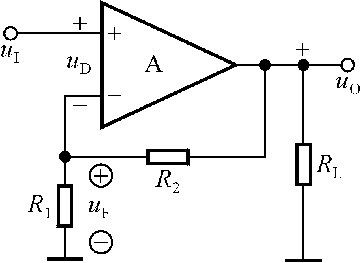
\includegraphics[width=0.4\textwidth]{fufankui1}}
			\subcaptionbox{电压并联负反馈电路\label{tu:2}}[6cm]{
			    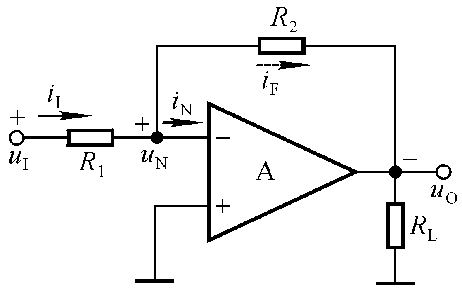
\includegraphics[width=0.4\textwidth]{fufankui2}}
			\subcaptionbox{电流串联负反馈电路\label{tu:3}}[6cm]{
				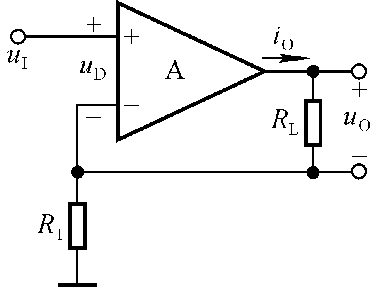
\includegraphics[width=0.4\textwidth]{fufankui3}}
			\subcaptionbox{电流并联负反馈电路\label{tu:4}}[6cm]{
				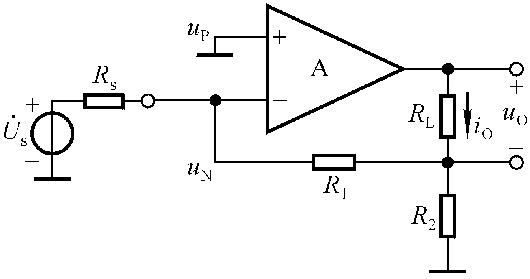
\includegraphics[width=0.4\textwidth]{fufankui4}}
		\end{figure}
		\begin{equation*}
			\dot{F}_{uu}=\frac{\dot{U}_{\rm{f}}}{\dot{U}_{\rm{o}}}=\frac{R_1}{R_1+R_2}
		\end{equation*}
		\item 电压并联负反馈电路见图~\ref{tu:2},容易得到
		\begin{equation*}
			\dot{F}_{iu}=\frac{\dot{I}_{\rm{f}}}{\dot{U}_{\rm{o}}}=-\frac{1}{R_2}
		\end{equation*}
		\item 电流串联负反馈电路见图~\ref{tu:3},容易得到
		\begin{equation*}
			\dot{F}_{ui}=\frac{\dot{U}_{\rm{f}}}{\dot{I}_{\rm{o}}}=R_1
		\end{equation*}
		\item 电流并联负反馈电路见图~\ref{tu:4},注意到电流的分流跟电阻成反比,容易得到
		\begin{equation*}
			\dot{F}_{ii}=\frac{\dot{I}_{\rm{f}}}{\dot{I}_{\rm{o}}}=-\frac{R_2}{R_1+R_2}
		\end{equation*}
	\end{enumerate}
    \item 下面分析四种负反馈的放大倍数,注意到反复使用了~\ref{eq:6}
    \begin{enumerate}
    	\item 电压串联负反馈电路的放大倍数
    	\begin{equation*}
    		\dot{A}_{uu\rm{f}}=\frac{\dot{U}_{\rm{o}}}{\dot{U}_{\rm{i}}}\approx\frac{\dot{U}_{\rm{o}}}{\dot{U}_{\rm{f}}}=\frac{1}{\dot{F}_{uu}}=1+\frac{R_2}{R_1}
    	\end{equation*}
    	\item 电压并联负反馈电路的放大倍数
    	\begin{equation*}
    		1
    	\end{equation*}
    \end{enumerate}
\end{enumerate}
\section{信号的运算与处理}
\section{波形的发生和信号的转换}
\section{功率放大电路}
\section{直流电源}
\subsection{直流电源组成}
	直流电源是由以下几个部分组成的(图~\ref{tu:5}~)
	\begin{figure}[htbp]
		\centering
		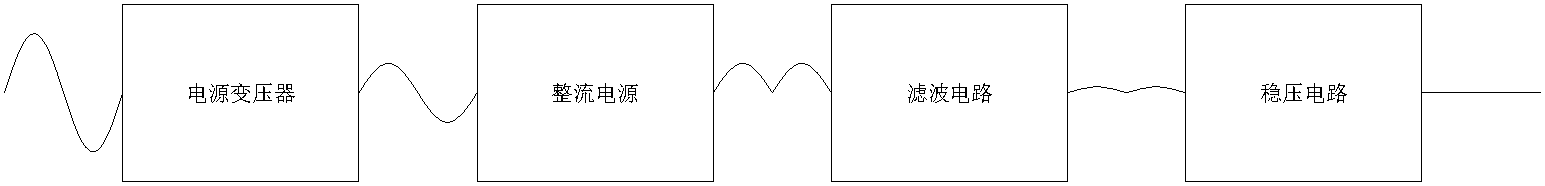
\includegraphics[width=1\textwidth]{tu5.pdf}
		\caption{直流电源组成说明图}\label{tu:5}
	\end{figure}
	变压器我们已经学过了,现在看看整流电路、滤波电路和稳压电路是干嘛的

	看最简单的单相半波整流电路(见图~\ref{tu:6}~)
	\begin{figure}[htbp]
		\centering
		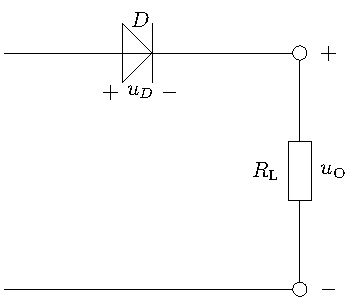
\includegraphics[width=0.5\textwidth]{tu6.pdf}
		\caption{单相半波整流电路}\label{tu:6}
	\end{figure}

	显然,图~\ref{tu:6}~所示电路的作用是截断一半的电流,那么我们来计算一下它的主要参数

	$u_{\mathrm{O}}$ 的平均值 $U_{\mathrm{O(AV)}}=$
\section{考试重点}
第一章 PN结、二极管、三极管、场效应管、MOS管

第二章 静态工作点、几种等效模型、几种参数的计算

第三章 多级放大电路静态/动态参数的计算、差分模块 $R_e$ , $R_L$ 的处理、互补输出级(克服交越失真)

第四章 由波特图写表达式及逆过程

第五章 负反馈组态、深度负反馈的计算

第六章 由图求运放关系及逆过程

第七章 正弦波振荡的判断

-RC 桥式振荡的计算(注意: $|F|=\frac{1}{3},|A_u|=3$)

-LC 振荡的判断(三种振荡电路)

--变压器考同名端标记

--其余考能否形成正反馈

-求阈值电压、画电压传输特性、根据传输特性画波形

第八章 OCL、OTL电路、计算 $P_{om},P_{V},\eta$ 、先判断是什么电路再套公式

第九章 整流、滤波、稳压
\end{document}